%File: anonymous-submission-latex-2024.tex
\documentclass[letterpaper]{article} % DO NOT CHANGE THIS
\usepackage[submission]{aaai24}  % DO NOT CHANGE THIS
\usepackage{times}  % DO NOT CHANGE THIS
\usepackage{helvet}  % DO NOT CHANGE THIS
\usepackage{courier}  % DO NOT CHANGE THIS
\usepackage[hyphens]{url}  % DO NOT CHANGE THIS
\usepackage{url}
\usepackage{graphicx} % DO NOT CHANGE THIS
\urlstyle{rm} % DO NOT CHANGE THIS
\def\UrlFont{\rm}  % DO NOT CHANGE THIS
\usepackage{natbib}  % DO NOT CHANGE THIS AND DO NOT ADD ANY OPTIONS TO IT
\usepackage{caption} % DO NOT CHANGE THIS AND DO NOT ADD ANY OPTIONS TO IT
\frenchspacing  % DO NOT CHANGE THIS
\setlength{\pdfpagewidth}{8.5in} % DO NOT CHANGE THIS
\setlength{\pdfpageheight}{11in} % DO NOT CHANGE THIS
\usepackage{enumitem}
%
% These are recommended to typeset algorithms but not required. See the subsubsection on algorithms. Remove them if you don't have algorithms in your paper.
\usepackage{algorithm}
\usepackage{algorithmic}

%
% These are are recommended to typeset listings but not required. See the subsubsection on listing. Remove this block if you don't have listings in your paper.
\usepackage{newfloat}
\usepackage{listings}
\DeclareCaptionStyle{ruled}{labelfont=normalfont,labelsep=colon,strut=off} % DO NOT CHANGE THIS
\lstset{%
	basicstyle={\footnotesize\ttfamily},% footnotesize acceptable for monospace
	numbers=left,numberstyle=\footnotesize,xleftmargin=2em,% show line numbers, remove this entire line if you don't want the numbers.
	aboveskip=0pt,belowskip=0pt,%
	showstringspaces=false,tabsize=2,breaklines=true}
\floatstyle{ruled}
\newfloat{listing}{tb}{lst}{}
\floatname{listing}{Listing}
%
% Keep the \pdfinfo as shown here. There's no need
% for you to add the /Title and /Author tags.
\pdfinfo{
/TemplateVersion (2024.1)
}
\usepackage{hyperref}
\usepackage[switch, modulo]{lineno}
\linenumbers





\setcounter{secnumdepth}{0} %May be changed to 1 or 2 if section numbers are desired.

% The file aaai24.sty is the style file for AAAI Press
% proceedings, working notes, and technical reports.
%

% Title

% Your title must be in mixed case, not sentence case.
% That means all verbs (including short verbs like be, is, using,and go),
% nouns, adverbs, adjectives should be capitalized, including both words in hyphenated terms, while
% articles, conjunctions, and prepositions are lower case unless they
% directly follow a colon or long dash
\title{Capturing Yale’s Campus: Geolocation Based On Visual Features}
\author{
    Linh Pham\equalcontrib,
    Eric Yoon\equalcontrib
}



\begin{document}

\maketitle

\begin{abstract}
Geolocation data is invaluable for researchers and photographers alike, but many images come without geolocation data due to messaging and social media apps removing the information for privacy purposes. While previous research has been conducted on re-constructing geolocation data from an image’s pixels, our approach focuses on a specific use-case of determining whether an image was taken at a prespecified location. To demonstrate this, we created a model that classifies whether an image was taken on Yale campus or not. To address the sparse and unlabeled nature of training photos taken on Yale campus, we propose three methods of data collection: (1) using public Instagram accounts, (2) using the Google Maps Places API, and (3) using our personal photo libraries. We then used transfer learning to develop a binary classification model, the best of which had a final test accuracy of 92\%. We observed that the model is generally able to recognize Yale-like scenery and architecture, but fails for some specific types of images.
\end{abstract}

\section{Background}
Geolocation metadata is particularly useful in images and is used in a variety of applications. Researchers rely on geolocation information to create specialized datasets; social media apps use geo-data for location-based features and recommendation algorithms; and everyday photographers rely on geo-data to organize their libraries. While most modern smartphone cameras automatically capture this data in machine-readable format, there are many cases in which this data can be lost. For example, when photos are uploaded to social media or messaging apps, EXIF and geolocation data are often stripped for privacy reasons. As such, recreating geolocation data from an image’s pixels alone is a task worth researching.

There have been previous approaches to recreating geolocation data, including using scene-matching[1] or deep neural networks[2]. However, these papers focused on geolocation on a global scale, attempting to identify an image taken anywhere in the world. Our approach attempts to trade versatility for accuracy—instead of asking a general question of “where is this image taken,” we attempt to see if a specialized model could be trained for a specific location that a data scientist has in mind.

Our project demonstrates how a binary classification model can be trained using publicly-available data to tell whether an image was taken in a specific region. To demonstrate this, we constructed a model that aims to tell whether an image was taken on Yale University campus. This project is as much about training a model as it is about finding an adequate volume of data. We present (a) three ways to find image data associated with a location, like a campus; and (b) an approach to training a binary classification model using transfer learning.

\section{Data Collection}
Yale Campus has been widely photographed, with many photos of campus taken and published online. However, there is no central repository of such photos; such a problem is true for other locations of interest of a similar nature. While many photos of Yale are published with associated keywords or hashtags, photos of architecture and landscapes are hard to distinguish from photos that do not depict the campus. An Instagram search for the hashtag '\#yale' gives plenty of examples of unhelpful images:

\begin{figure}
    \centering
    \includegraphics[width=1\linewidth]{pic1.png}
    \caption{Unhelpful Yale Images}
    \label{fig:enter-label}
\end{figure}

As such, keyword or hashtag searches by themselves cannot provide a clean repository of campus images. We instead detail three methods we used to obtain 1000+ images of Yale campus.


\subsection{Instagram}
We discovered an Instagram account, '@yale\_vibes', that solely posts pictures of Yale campus. Using a Chrome browser extension called “Mass Download for Instagram,”[3] we were able to download each photo.

While this dataset contained around ~500 photos of Yale campus, there were some traits that could decrease the robustness of our model. First, the account is run by three students, making it likely that many photos were taken with the same model of camera. This could result in our model paying attention to the cameras’ unique traits and artifacts instead of the features of the campus. Additionally, these photos appear to be enhanced and edited, which could also result in our model classifying any photos edited in a similar fashion as Yale campus images. As such, we decided to augment our dataset with more sources of images. 

\begin{figure}
    \centering
    \includegraphics[width=1\linewidth]{pic2.png}
    \caption{Examples of images downloaded from Instagram account $\text{@yale\_vibes}$}
    \label{fig:enter-label}
\end{figure}


\subsection{Google Maps}
Google Maps provides a Places API [4] that allows developers to retrieve data, including user-contributed images, of places on Google Maps. Our first approach was to use this Places API to fetch images of the location titled “Yale University.” However, the API only allows 10 images to be fetched per place, so this approach wouldn’t allow us to get more than 10 images.

We were able to obtain a list of on-campus buildings published by Yale [5]. Using the Places API text search endpoint, we found the Google Maps listing for each of these building names. Then, we fetched the first 10 images of each building. This method resulted in a total of ~700 images of Yale campus, taken by Google Maps users.

Since these images were crowdsourced by Google Maps, they represented a wide range of camera models and editing styles, unlike our Instagram dataset.

\begin{figure}
    \centering
    \includegraphics[width=1\linewidth]{pic3.png}
    \caption{Examples of images taken from Google Maps}
    \label{fig:enter-label}
\end{figure}

\subsection{Personal Photo Libraries}
As Yale University students ourselves, we had many photos in our personal photo libraries that were taken on Yale campus. We decided to use these images to augment our dataset.

To facilitate the filtering process of photo libraries hosted in Google Photos, we created a program that could filter out images taken on Yale campus. The owner of a photo library is able to create a Google Takeout export of their Google Photos library, which includes .json files with metadata including geolocation latitude/longitude. Using a Python script, we were able to read this metadata and determine which photos were taken on Yale campus. Additional manual filtering was necessary to select for only photos of landscapes and architecture (as opposed to photos of people), but the filtering program greatly reduced the human workload necessary.

Out of 6122 photos in Eric’s Google Photos library, 339 were taken on Yale Campus. Of these, 76 were deemed usable.

Out of 2,452 photos in Linh’s Apple Photos library, 42 were deemed usable. (Most of her images were of her cat on campus, and very few of the actual campus itself.) Linh further collected 88 images of Yale campus from friends.

We decided to use these images from personal photo libraries to test the model under real-world conditions, rather than including it in our train/test/validate dataset. 

\begin{figure}
    \centering
    \includegraphics[width=1\linewidth]{pic4.png}
    \caption{Examples of images taken from personal photo libraries}
    \label{fig:enter-label}
\end{figure}



\subsection{Non Yale Photos}
To train our binary classifier, we needed photos of landscapes and architecture that were NOT taken on Yale campus. We used the publicly-available Places365 [6] dataset to provide negative examples. Due to the small number of Yale images we had, we only needed a similar small number of non-Yale images; as such, we decided to use the Places365 validation set rather than the full set. We further filtered by label, only choosing photos that were similar to the ones we would see on Yale campus; examples include dorm room, office building, and dining hall. 

\begin{figure}
    \centering
    \includegraphics[width=1\linewidth]{pic5.png}
    \caption{Examples of images from the Places365 dataset}
    \label{fig:enter-label}
\end{figure}

\section{Classification Training}
\subsection{Training without Transfer Learning}
We first attempted to train the model without using transfer learning. Both VGG and ResNet architectures failed to converge. When trained on an equal number of Yale and non-Yale images, our accuracy stayed at almost exactly $50\%$, even after 10 epochs of training. When we changed the ratio of Yale to non-Yale images, we noticed the accuracy also changed to match the ratio, indicating that the model was learning to always classify as non-Yale. As such, we decided to change our approach to take advantage of transfer learning.

\subsection{Transfer Learning}
Training a model from scratch is a time consuming process, and in the age of modern technology, can be considered redundant. This is where Transfer learning comes in. Transfer learning refers to the process of utilizing pre-trained models and modifying it slightly, in order to achieve the desired result. There are different methods of transfer learning, which depend on both the size and similarity of the dataset. This dataset was about moderately sized, but we considered the similarity to be high, as the differentiation between Yale architecture and other architecture is nuanced and complex. We primarily utilized a TensorFlow tutorial to help with code development [7]. More detail on the code can be found in the tutorial, but we provide a quick summary of our process. 



\noindent\textbf{--- Part 1 ---}
\begin{itemize}
    \item Data download and augmentation
\end{itemize}
\textbf{--- Part 2 ---}
\begin{itemize}
    \item Base model - either VGG or MobileNetV2
    \begin{itemize}
        \item Freeze convolutional base
        \item Feature extraction
    \end{itemize}
\end{itemize}
\textbf{--- Part 3 ---}
\begin{itemize}
    \item Fine Tuning: Where as before we only trained the few layers we added at the top of the base model, we are now updating the weights throughout the first few layers of the pretrained model.
    \begin{itemize}
        \item Unfreeze and train from layer 100 and onwards
    \end{itemize}
\end{itemize}


\subsubsection{Part 1}
We downloaded 1200 images from Place365 for our “non-Yale” classification. We applied an initial resize transformation of 500 x 500 as well as a conversion to a Tensor. We then applied data augmentation, specifically horizontal flips and rotation scaling in order to create more training images. This also helps in feature extraction. 

\subsubsection{Part 2}
Then, we loaded in our base model (either VGG or MobileNetV2). We froze the convolutional base to prevent training of the transferred initial layers. Afterwards, we added a classification layer and a pooling layer to help classify images. We then trained for 10 epochs on this first part. 

\subsubsection{Part 3}
After 10 epochs, we then started fine tuning the model. We unfroze the transferred initial layers, allowing them to further train.

\section{Analysis}

\subsection{MobileNetV2}

\begin{figure}[h!]
    \centering
    % First image
    \begin{minipage}{0.2\textwidth}
        \centering
        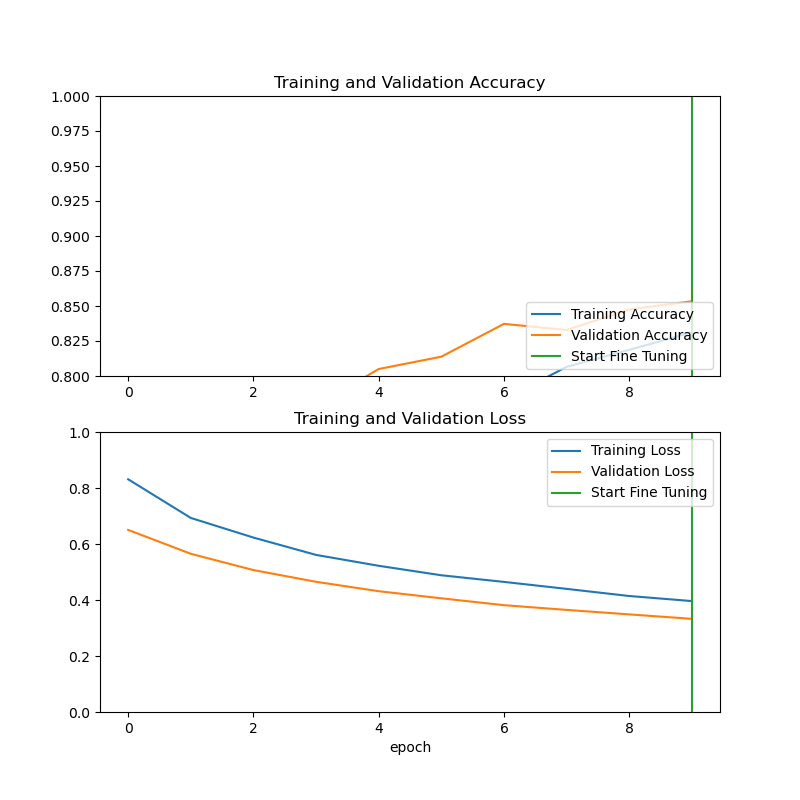
\includegraphics[width=\textwidth]{imagenet_acc_loss_1.png}
        \caption{Accuracy and loss before fine-tuning}
        \label{fig:fig1}
    \end{minipage}
    \hfill
    % Second image
    \begin{minipage}{0.2\textwidth}
        \centering
        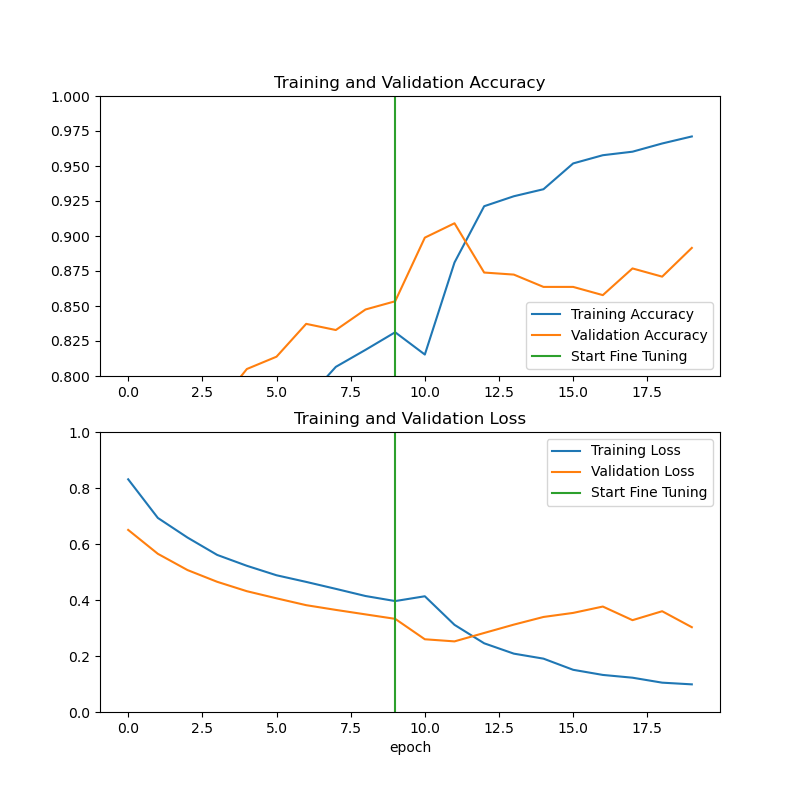
\includegraphics[width=\textwidth]{imagenet_acc_loss_2.png}
        \caption{Accuracy and loss for first part after fine-tuning}
        \label{fig:fig2}
    \end{minipage}
\end{figure}


Figure 6 shows the accuracy and loss for the first part of training, when we only added a classification task to the pretrained model. We can see that accuracy increases for both the training and validation set. This is an indicator of convergence, showing that our transfer learning approach is learning the data. After doing some research online, we found that the training accuracy is likely higher than validation accuracy as a result of using dropout [8].

In Figure 7, we can see that the training accuracy starts to surpass validation accuracy. The validation loss also rapidly increases and then remains above the training loss. This indicates some level of overfitting, with the model memorizing the training data rather than learning to identify features. However, the gap is decreasing with the amount of training; thus, it is plausible that after more epochs, the model would start to generalize better. 

\subsection{VGG16}

\begin{figure}[h!]
    \centering
    % First image
    \begin{minipage}{0.2\textwidth}
        \centering
        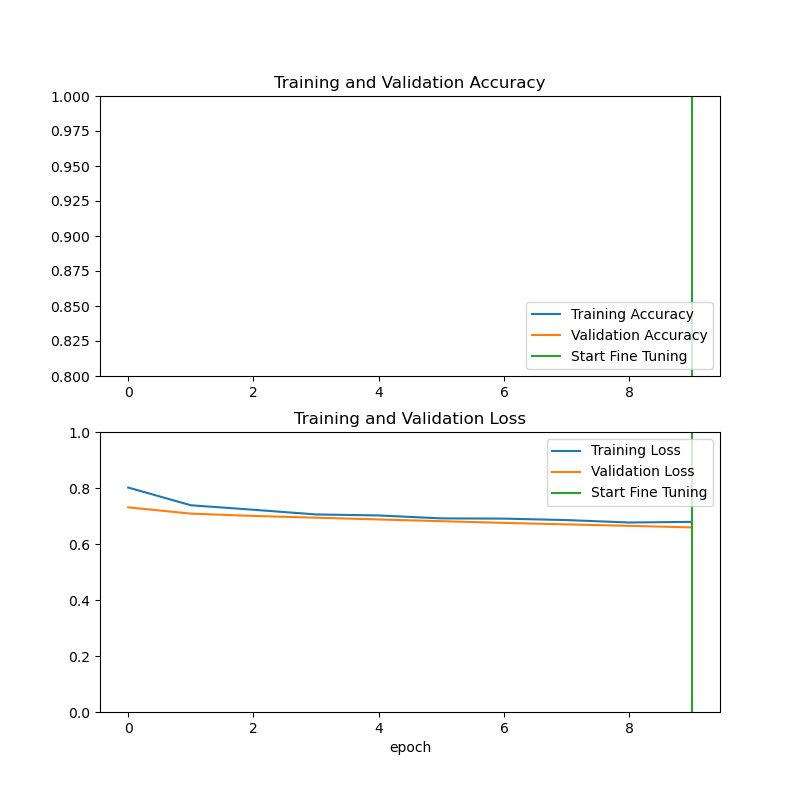
\includegraphics[width=\textwidth]{vgg16_acc_loss_1.png}
        \caption{Accuracy and loss before fine-tuning}
        \label{fig:fig1}
    \end{minipage}
    \hfill
    % Second image
    \begin{minipage}{0.2\textwidth}
        \centering
        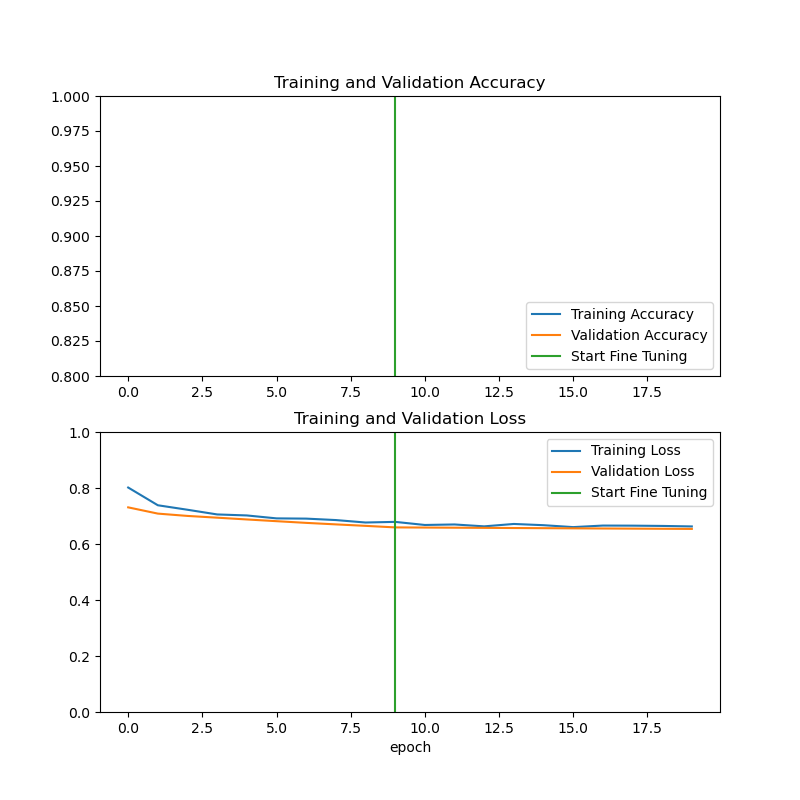
\includegraphics[width=\textwidth]{vgg16_acc_loss_2.png}
        \caption{Accuracy and loss for first part after fine-tuning}
        \label{fig:fig2}
    \end{minipage}
\end{figure}


In Figure 8 we can see that the training accuracy and validation accuracy remain relatively close in the beginning. Though these are not smooth curves, it indicates the model is learning well. 

In Figure 9 we can see that training and validation accuracy starts to divide a little more. Both accuracies flatline, indicating an upper bound to the accuracy with respect to amount of training. Unlike VGG16, the validation accuracy remains above the training accuracy, and the validation loss remains below the training loss. 

\section{Results}

Our final test accuracy for MobileNetV2 was $92\%$. While this seems like a success, the results from our loss and accuracy suggest overfitting. There are two ways to resolve this problem. We can add even more images, or go through our data again to make identifiable features of Yale. We acknowledge that our classification task is quite a complex one. While a classifier that differentiates, for example, architecture from scenery may have a high accuracy, our classifier differentiating Yale architecture from non-Yale architecture is a significantly harder task. Additionally, Yale has varied architecture, so the question is not as simple as classifying Gothic-style architecture as “Yale” and others as “non-Yale.” For such a complex task, we believe adding more layers, or more importantly, adding more training data would allow our model to perform better.

The test accuracy for VGG16 was $65\%$. MobileNetV2 is a model meant for mobile applications, thus it is lighter and faster, but focuses less on actual accuracy. MobileNetV2 has about 4 million parameters and ~314 million FLOPS, but in comparison, the VGG16 model has about 138 million parameters and ~15 billion FLOPS. While VGG16 focuses on accuracy and training, MobileNetV2 chooses to sacrifice accuracy for speed. VGG16 is able to maintain high validation accuracy [Figure 4], indicating that it does not overfit. This is important as both VGG16 and MobileNetV2 trained on the same amount of images. Thus, the issue is not the lack of data, but on model construction. One way to improve the accuracy for VGG16 would probably be to train for longer. While 20 epochs was relatively fine for MobileNetV2, 20 epochs was most likely low for VGG16 due to the increased complexity of the model.


\subsection{Real World Testing}

Using our saved model checkpoints, we were able to test our model on images that were not included anywhere in our train/test/validate dataset. We observed a high sensitivity but a low specificity. We manually chose a classification boundary of 0.9 based on our own observations, although we acknowledge that this could have been chosen more empirically.

In a collection of 236 images that were taken in 2022 from Eric’s photo library (before Eric entered Yale), 118 were predicted to be Yale and 118 were predicted to be non-Yale.

In a collection of 76 hand-picked images of Yale scenery from Eric’s photo library, 63 were predicted to be Yale and 13 non-Yale.

Here are some examples of true positives, true negatives, false positives, and false negatives.
\begin{figure}
    \centering
    \includegraphics[width=1\linewidth]{pic6.png}
    \caption{True Positives (actual Yale, predicted Yale)}
    \label{fig:enter-label}
\end{figure}

\begin{figure}
    \centering
    \includegraphics[width=1\linewidth]{pic7.png}
    \caption{False Negatives (actual Yale, predicted non-Yale)}
    \label{fig:enter-label}
\end{figure}

\begin{figure}
    \centering
    \includegraphics[width=1\linewidth]{pic8.png}
    \caption{True Negatives (actual non-Yale, predicted non-Yale)}
    \label{fig:enter-label}
\end{figure}

\begin{figure}
    \centering
    \includegraphics[width=1\linewidth]{pic9.png}
    \caption{False Positives (actual non-Yale, predicted Yale)}
    \label{fig:enter-label}
\end{figure}

After manually inspecting all false negatives, we determined that these were “understandable” errors, as most of the false negative images were (a) nighttime photos, (b) photos with people in the foreground, or (c) photos of interiors (rather than exteriors).

After manually inspecting false positives, we also understood why the model classified these as Yale images. Most of the false positives were landscapes; this indicates that the model may have learned to identify landscapes rather than Yale architecture.

\section{Conclusion}
We conclude that due to the complex nature of this task, and the limited availability of public data, creating a Yale vs. non-Yale classifier is extremely difficult. However, the task seems possible, as our model was able to classify images with a significant accuracy percentage. Our techniques to obtain data proved to be useful, and we stand by our choice to use transfer learning.

\section{Additional Resources}
You can view our code in our \href{https://github.com/EricYale/EENG439-Final-Project}{public GitHub repository}.

Please install all requisite packages using pip3 before using our code.

\begin{itemize}
    \item \texttt{data\_scraping/google\_maps/maps.ipynb}: Interactive notebook to get data from the Places API.
    \item \texttt{data\_scraping/google\_photos/photos.ipynb}: Interactive notebook to extract Yale images from a Google Takeout export.
    \item \texttt{data\_processing.py}: Download non-Yale Places365 images; format images into the correct file structure and dimensions.
    \item \texttt{interactive\_classifier.py}: Run our trained model on an image of your choice.
    \item \texttt{train\_imagenet.py}: Train the MobileNet model from scratch.
    \item \texttt{train\_vgg.py}: Train the VGG model from scratch.
\end{itemize}

\begin{thebibliography}{99}

\bibitem{hays2008}
Hays, James, and Alexei Efros. \textit{IM2GPS: Estimating Geographic Information from a Single Image}. \url{http://graphics.cs.cmu.edu/projects/im2gps/im2gps.pdf}.

\bibitem{weyand2016}
Weyand, Tobias, et al. “PlaNet - Photo Geolocation with Convolutional Neural Networks.” \textit{Lecture Notes in Computer Science}, Springer Science+Business Media, Jan. 2016, pp. 37–55, \url{https://doi.org/10.1007/978-3-319-46484-8_3}. Accessed 14 Dec. 2024.

\bibitem{massdownloader}
“Download Instagram Stories - Mass Downloader for Instagram.” \textit{Mass-Downloader.com}, 2024, \url{https://mass-downloader.com/}. Accessed 14 Dec. 2024.

\bibitem{googleplaces}
“Places API Overview.” \textit{Google for Developers}, 2024, \url{https://developers.google.com/maps/documentation/places/web-service/overview}. Accessed 14 Dec. 2024.

\bibitem{yale}
“Building Abbreviations < Yale University.” \textit{Yale University}, 2024, \url{https://catalog.yale.edu/ycps/building-abbreviations/}. Accessed 14 Dec. 2024.

\bibitem{places365}
“CSAILVision/Places365: The Places365-CNNs for Scene Classification.” \textit{CSAIL Vision}, 2024, \url{https://github.com/CSAILVision/places365}. Accessed 14 Dec. 2024.

\bibitem{tensorflow}
“Transfer Learning and Fine-Tuning.” \textit{TensorFlow}, 2024, \url{https://www.tensorflow.org/tutorials/images/transfer_learning}. Accessed 14 Dec. 2024.

\bibitem{stackoverflow}
“Higher Validation Accuracy, than Training Accuracy Using TensorFlow and Keras.” \textit{@yhenon on StackOverflow}, 15 May 2017, \url{https://stackoverflow.com/questions/43979449/higher-validation-accuracy-than-training-accuracy-using-tensorflow-and-keras/43982656#43982656}. Accessed 14 Dec. 2024.

\end{thebibliography}


\end{document}
